\documentclass[conference]{IEEEtran}
\IEEEoverridecommandlockouts
% The preceding line is only needed to identify funding in the first footnote. If that is unneeded, please comment it out.
\usepackage{cite}
\usepackage{amsmath,amssymb,amsfonts,bm,physics}
\usepackage{algorithmic}
\usepackage{graphicx}
\usepackage{caption}
\usepackage[list=true,labelformat=simple]{subcaption}
\captionsetup[sub]{skip=2pt}
\renewcommand\thesubfigure{(\alph{subfigure})}
\usepackage{textcomp}
\usepackage{xcolor}
\usepackage[colorinlistoftodos]{todonotes}
\usepackage{siunitx}
\usepackage{nohyperref}

\def\BibTeX{{\rm B\kern-.05em{\sc i\kern-.025em b}\kern-.08em
    T\kern-.1667em\lower.7ex\hbox{E}\kern-.125emX}}
\begin{document}

\title{ Towards the Development of an Intelligent Building Energy Management System -- iBEMS
  \thanks{The results presented in this paper were produced by a group of senior
    undergraduate students: Brian Lauer and Elliot Watkins }
}

\author{\IEEEauthorblockN{Brian Lauer, Elliot Watkins, and Md Suruz Miah}
\IEEEauthorblockA{\textit{Department of Electrical and Computer Engineering} \\
\textit{Bradley University}\\
Peoria, Illinois, United States of America \\
\{blauer, ejwatkins\}@mail.bradley.edu, smiah@bradley.edu}
}

\maketitle

\begin{abstract}

  Smart building energy management and/or monitoring has recently emerged as a
  promising task due to global climate change issues. Such a task has received
  thorough attention for the advent of emerging Internet-of-Things (IoT)
  technology. Numerous building energy management systems are commercially
  available in the market. Most of them lack modularity or are driven by an
  overwhelming degree of manual configurations for performing building
  automation. In this paper, we present the development of a modular IoT-based framework for an intelligent building energy management system (iBEMS). The proposed framework is open-source and leverages the features of decentralized multi-agent systems. The principal component of the framework is the BEMS core that implements building automation features, such as an optimal scheduler, displaying weather information, detecting new IoT devices, monitoring energy consumption, and remotely controlling operation of IoT devices.
  
\end{abstract}

\begin{IEEEkeywords}
  mobile robots, navigation, radio frequency identification, robotic cart 
\end{IEEEkeywords}

\section{Introduction}
\label{sec:introduction}

The Internet of Things (IoT) is a large network of embedded devices such as sensors, wearables, and appliances capable of receiving control commands and reporting
data over the Internet. Many industries take advantage of this infrastructure to
improve process flow and efficiency. One of these industries is the commercial
and industrial sector which often employ building automation or management
systems to help better manage processes or devices in a building like air
conditioning systems, lights or industrial machines. Technological advancements
have allowed devices to become connected to a building network through
communication protocols like WiFi, Ethernet, Modbus, or BACnet which enables
them to be more easily controlled from a central system.


The overall goal of this work is to create a platform in which users can login and access devices
connected to a building's energy supply. This will allow the user to closely
monitor energy usage throughout a commercial or residential building.
Additionally, the user will be able to control devices connected to the
platform, allowing precise control over the building's energy use. The minimum
viable product of this project will be to connect to 1 to 3 devices via the the
platform and control them.

% The previous senior project group worked on creating a remote motor control system with a Raspberry Pi and XBee module. To supply power directly to the motor and XBee with a single power supply, they used a buck-boost converter capable of stepping down power supply voltage to 3.3 V. They implemented a Python script that uses the Linux command \texttt{nmap} to search for the Raspberry Pi on the network. The Raspberry Pi connects to the transmitter XBee via a serial connection to transmit commands to the receiver XBee mounted to the motor. They were able to simply toggle the motor on and off and partially implemented this functionality in BEMOSS (Building Energy Management Open Source Software). A second portion of their project was implementing an HVAC control algorithm capable of controlling the temperature of a home with the Linear Quadratic Regulator control algorithm.

% During a research project led by Miah \textit{et al.,} the DC motor interface was successfully
% implemented into the BEMOSS platform which required adding a great deal of source code
% to the platform to fully implement the device as BEMOSS does not support adding
% new devices currently. The research also consisted of adding new
% features such as a logo to the
% platform for the motor. A possible improvement our platform will make is helping
% developers on the project add new devices more easily.

% One of the improvements our project makes over the previous is the use of UDP (user datagram protocol) multicasting which does not require any superuser privileges to locate an
% embedded computer (Beaglebone Blue, for example). This implementation is also more convenient
% because it does not require installing any packages as multicasting is natively
% supported by most embedded Linux systems. If in the future, multiple embedded
% computers are needed to be discovered, the multicasting system works elegantly
% as each device can simply listen on a provided multicast group which consists of
% an IP address and port number.

A great deal of research has been conducted in the field of building energy
management. Multiple different platforms have been developed that demonstrate
the vast amount of features and possibilities that exist in developing these
types of software. One such platform is
BEMOSS\footnote{\href{https://www.bemoss.org}{https://www.bemoss.org}} (Building
Energy Management Open Source Software) from the Virginia Polytechnic Institute
and State University Advanced Research Institute. BEMOSS features include being
open-source, allowing for multiple communication technologies, and supporting
many common IoT devices. This system allows for monitoring and controlling a
variety of devices securely.

Another open-source platform is rEMpy or residential Energy Management in
Python~\cite{FAGIANI2018131}. The main focus of this platform developed by a team of researchers at
Universit\`{a} Politecnica delle Marche in Ancona, Italy was to simulate the
energy flow of a residential home. With the data collected from simulations, it
was possible for them to use forecasting and prediction algorithms to predict
various quantities such as energy usage and power consumption over a given time period. Their energy management system consists of a well-defined structure with components like a user interface, database, and optimal scheduler that communicate with modules like a prediction and thermal model. In terms of software technologies, it uses the Django web framework which provides a lot of built-in functionality for web development like a user-authentication system and object-relational mapping. Adapting the project to this framework could be a great way to help improve security and optimize database queries~\cite{fagiani2017}.

Authors in~\cite{Mayer2017} discusses Model Predictive Control (MPC)
which is a modern process control algorithm capable of taking into account
current and previous time values to improve building
automation. A multilevel hierarchy is presented to split
control of a building into two levels: the energy supply level and user level.
Example usage of this control scheme provided are temperature control of a
building and its corresponding zones and interaction with a smart grid. Studies
were performed on a commercial building with the building's energy supply system
and hierarchy model predictive controller implemented in Matlab.

In~\cite{8246800}, authors describe similar functional requirements to our
own BEMS Core. They periodically gather power consumption and device status data
and send that data to a database. The communication with devices
and power consumption reports are to be accessible through a web-based
application that is easy to use. The implementation of the iBEMS platform presented herein is simple and very
intuitive for the end-user.  

A control scheme in~\cite{Barchi2018} is presented to manage a photovoltaic
array and battery energy storage system. Tests were conducted in a shopping mall
with an electronic load to emulate the power consumption of the building.
Potentially, a similar technique could be used to model the energy demand of a
house in Simulink or Simscape model. Through their scheme, an intelligent BEMS
is used to collect measurable data such as power, voltage, and current and stored for offline analysis later. Their platform collects data every five minutes compared to the 20 second polling rate currently configured in our platform. A control algorithm was presented proving that grid energy is consumed more heavily during periods of low power demand rather than PV power.



The ultimate goal of the current work is to design and develop a new building energy management
platform incorporating learning, control, and estimation strategies, which is expected to remedy the
shortcomings of some existing platforms, BEMOSS, for instance.

\section{iBEMS Architecture}
\label{sec:iBEMS-Architecture}

At the center of the iBEMS architecture is the iBEMS core. This core interacts
with multiple peripherals including IoT devices and a weather API over the
internet. In this work, we developed the iBEMS to support for two 
IoT devices displayed in the high-level architecture shown in Fig.~\ref{fig:highLevelArchitecture}. %
%
\begin{figure}[htbp]
  \centering
  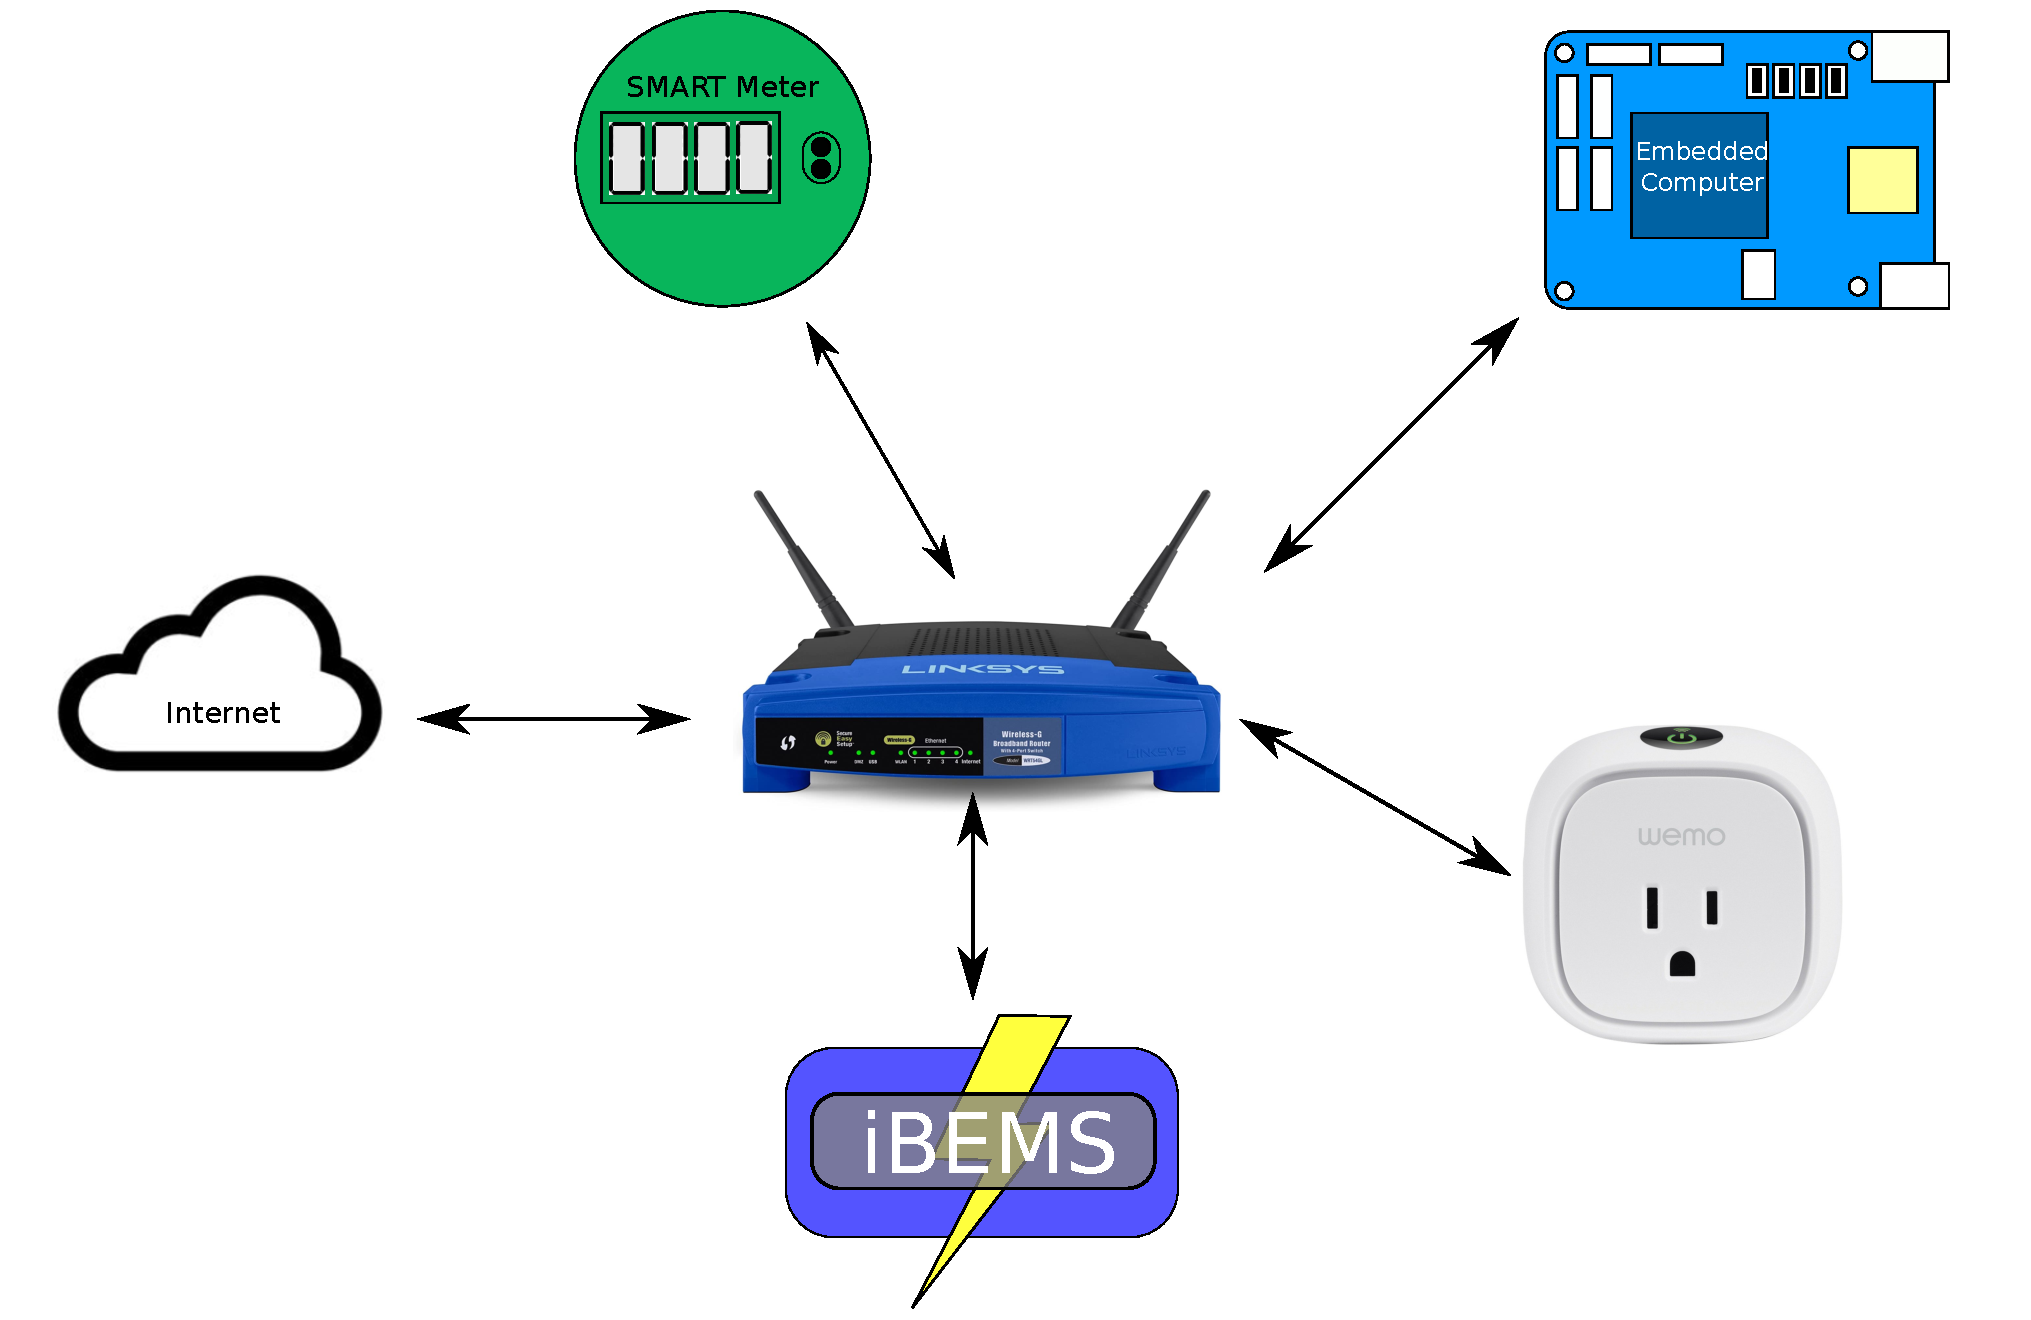
\includegraphics[scale=0.15]{figs/overallConnectionDiagram.pdf}
  \caption{High-level architecture of the proposed iBEMS.}
  \label{fig:highLevelArchitecture}
\end{figure}
%
These devices are the WeMo Insight Switch and an embedded computer known as the Beaglebone
Blue.  The core is also able to
connect the internet to download weather data for a local city through
OpenWeatherMap. Fig.~\ref{fig:functional_bd} gives the lower level functional block diagram of the system
architecture. %
%
\begin{figure}[htbp]
  \centering
  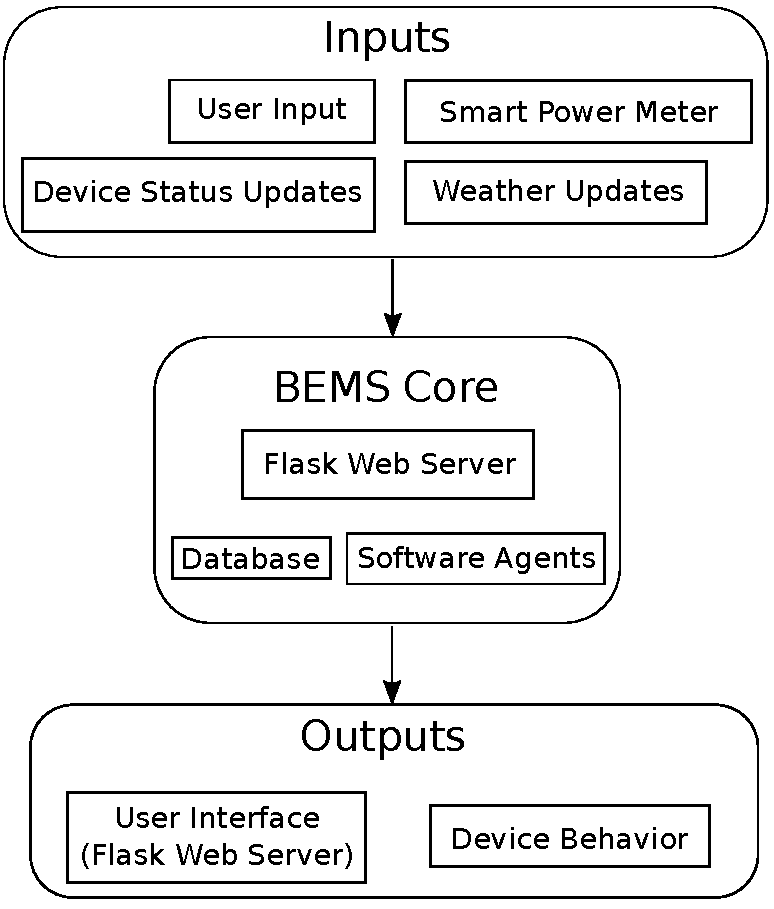
\includegraphics[scale=0.15]{figs/functionalBlockDiagram.pdf}
  \caption{Functional Block Diagram}
  \label{fig:functional_bd}
\end{figure}
%
The inputs include the user input through the web server, the device status
updates (On/Off, power usage, etc...) and the weather data. The iBEMS Core
itself consists of a Flask Web Server, 2 databases (Apache Cassandra and
SQLite), and 3 software agents (Discovery, Control, and Scheduling).


The Flask web server is built using a Python web framework titled Flask which
allows programmers to develop a dynamic web server capable of rendering data to
HTML pages. The benefit of this framework over other Python web frameworks like
Django is the large amount of customization available. For example, the
developers can create a completely custom user login system. For now, the server
is capable of being accessed only on the server computer running Ubuntu Linux.
In the future, support could be added to allow any user on the LAN to access the
web server. Other web frameworks use object relational mapping directly to
access the relevant databases. However, the current iBEMS uses direct queries with both
SQLite and the Cassandra query language to query the databases. We used
2 different databases to store information on. The Apache Cassandra database was
better suited for the time series data such as device status and power usage.
This database was therefore utilized a lot by the Control and Scheduling Agents.
The SQLite database hold parameters that do not change over time like device
ID's, IP addresses, and MAC addresses which made it amendable to the processes
in the Discovery Agent. The first agent that is
used by the iBEMS Core on startup is the discovery agent. It is responsible for
reaching out on the network and finding all devices that the iBEMS Core has
support for. This process involves retrieving the following parameters: IP
address, Port number, MAC address, Manufacturer, Name, and API. Once all
available devices are connected, the Control agent is used to change the status
of each device and collect power usage data in real time. Finally, the
scheduling will take input from the user and place the corresponding scheduling
periods in the Apache Cassandra database. Then, a thread is created to poll the
current device status at regular intervals and update the status if it does not
match the defined status in the Apache Cassandra database.


Fig.~\ref{fig:systemComponentInterconnection} provides an explanation of how
the components of the system interact with each other. %
%
\begin{figure}
  \centering
  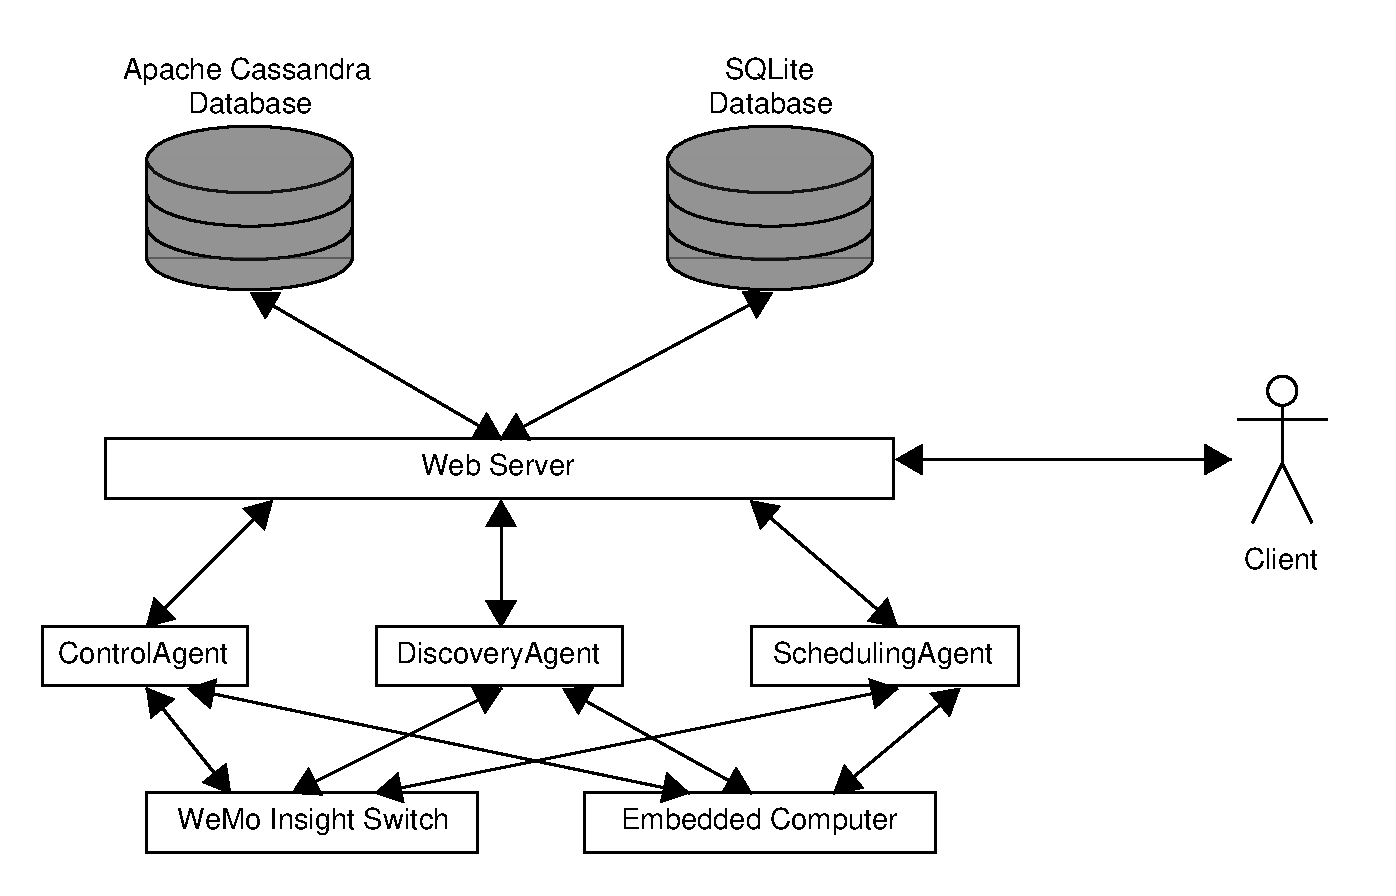
\includegraphics[scale=0.15]{figs/overallDiagram.pdf}
  \caption{Interconnection between system components}
  \label{fig:systemComponentInterconnection}
\end{figure}
%
The Apache Cassandra database and SQLite database are accessible from the web server, control agent, discovery agent, and scheduling agent. The web server queries the time series database and metadata database for vastly different purposes. Power plotting requires querying the Apache Cassandra database. To distinguish between the different devices on the front end, the metadata database is used. The agents utilize the Apache Cassandra database for storing and extracting time-series data. The agents use the metadata database to distinguish between different devices. 




% There are five general modes of operation in iBEMS shown in Fig.~\ref{fig:operationalModes}. In Mode 0, before iBEMS is even launched, the user must open the Startup Menu, which is a desktop graphical user interface (GUI). This is a simple GUI with only 2 buttons for starting and stopping iBEMS. Upon clicking \say{Start iBEMS}, the login page will load where the user can enter a valid username and password to use iBEMS. Once a valid username and password is entered, the home screen will be shown which displays the weather data being downloaded from the OpenWeatherMap API. This information includes temperature in Fahrenheit and Celsius, wind speed in MPH, humidity, and cloud coverage. At this point, a navigation bar is available to view the \say{Active Devices} page and the \say{Scheduling} page. \say{Active Devices} corresponds to Mode 3 for controlling devices in real time. The user will also be able to view power plots in this mode as well. Lastly, the \say{Scheduling} page is Mode 4 for creating schedules for all connected devices.



% \begin{figure}
%   \centering
%   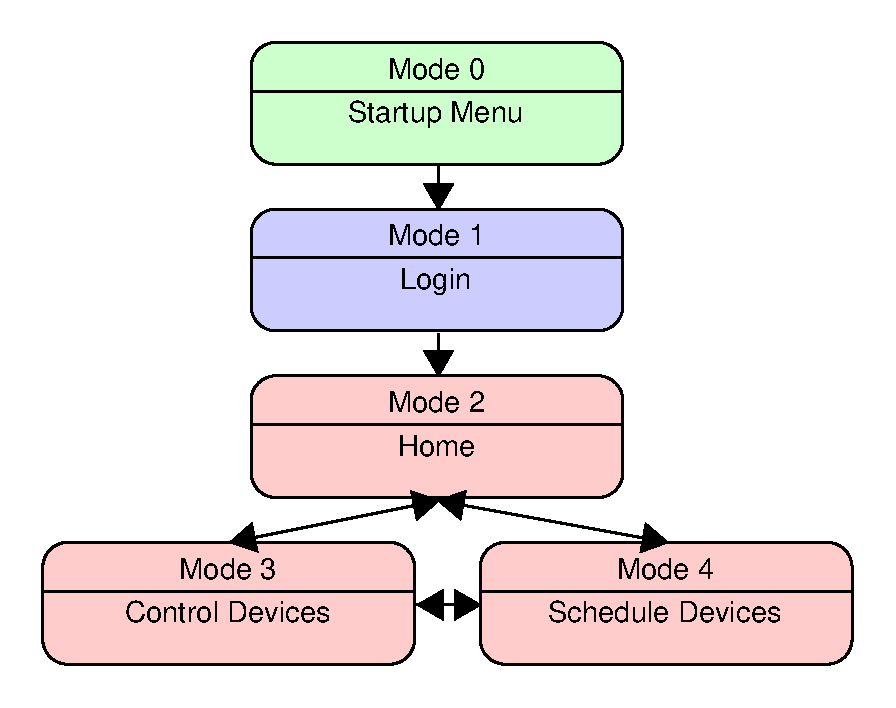
\includegraphics[scale=0.4]{figs/operationalModes.pdf}
%   \caption{Operation Modes Interaction}
%   \label{fig:operationalModes}
% \end{figure}

% \section{Hardware}

% A large feature of this project was being able to record power usage from the
% connected IoT devices. The embedded computer does not have a built-in capability
% to measure its own power usage, so a circuit was needed to make that
% possible. Essentially, this circuit will measure the current being used to drive
% one of the motors on the robot chassis. The on-board Analog-to-Digital-Converter
% (ADC) can be used to read the voltage across the resistor and since the
% resistance is known, the current can be calculated as $I = V/R$. Also, the
% voltage from the H-Bridge to drive the motors on the embedded computer is known
% so the power consumed by 1 motor is $Motor Drive Voltage * I$. For the specific
% robot chassis used in this project, there are 4 motors, so multiplying the power
% found from this circuit by 4 will give an approximation of the total power used
% by the robot. See Figure~\ref{fig:motorInterfaceCircuit} for details of the interface
% circuit for computer power usage by the DC motor. Also see Figure~\ref{fig:bb_connections} for how the circuit is connected to the embedded computer and robot chassis.

% \begin{figure}[H]
%   \centering
%   \begin{circuitikz}[american]
%     \tikzstyle{every node} = [font = \tiny]
%     % \usetikzlibrary{patterns}
%     \draw
%     (0,0) to[sqV,invert,l=Motor Drive Voltage from H-Bridge] ++(0,4*\smgrid)
%     to[Telmech=M,n=motor,fill=red!20] ++(4*\smgrid,0)
%     to[C,l=$1~{[}\mu F{]}$,*-*] ++(0,-4*\smgrid) to[short]++(-4*\smgrid,0); 
%     \draw
%     (4*\smgrid,4*\smgrid) to[short,-*]++(3*\smgrid,0)
%     to[short,-o]++(2*\smgrid,0)node[right]{Embedded Computer ADC (Ch\#0)};
%     \draw
%     (7*\smgrid,4*\smgrid) to[R,l=$2~{[}\Omega{]}$,-*]++(0,-4*\smgrid)
%     to[short]++(-4*\smgrid,0);
%     \draw
%     (7*\smgrid,0) to[short,-o]++(2*\smgrid,0) node[right]{Embedded
%       Computer ADC (Ground)};
%   \end{circuitikz}
%   \caption{Interface circuit to calculate power consumption of a DC motor
%     running from the embedded computer copmuter.}
%   \label{fig:motorInterfaceCircuit}
% \end{figure}

% \begin{figure}[H]
%     \centering
%     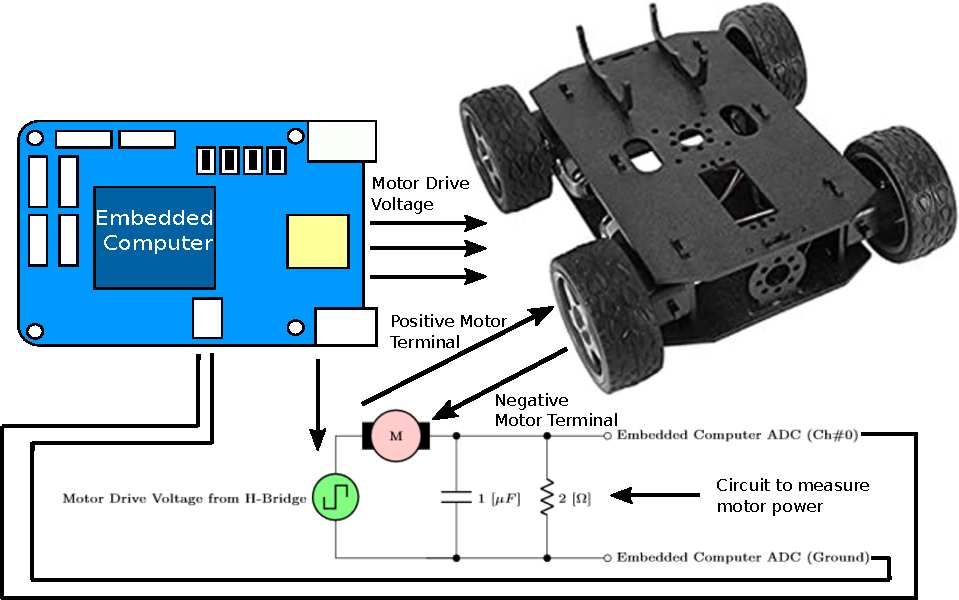
\includegraphics[scale=0.6]{figs/beaglebone/connections.pdf}
%     \caption{Connections between Embedded Computer, circuit, and robot chassis}
%     \label{fig:bb_connections}
% \end{figure}

% % \pagebreak
% \begin{figure}[H]
%     \centering
%     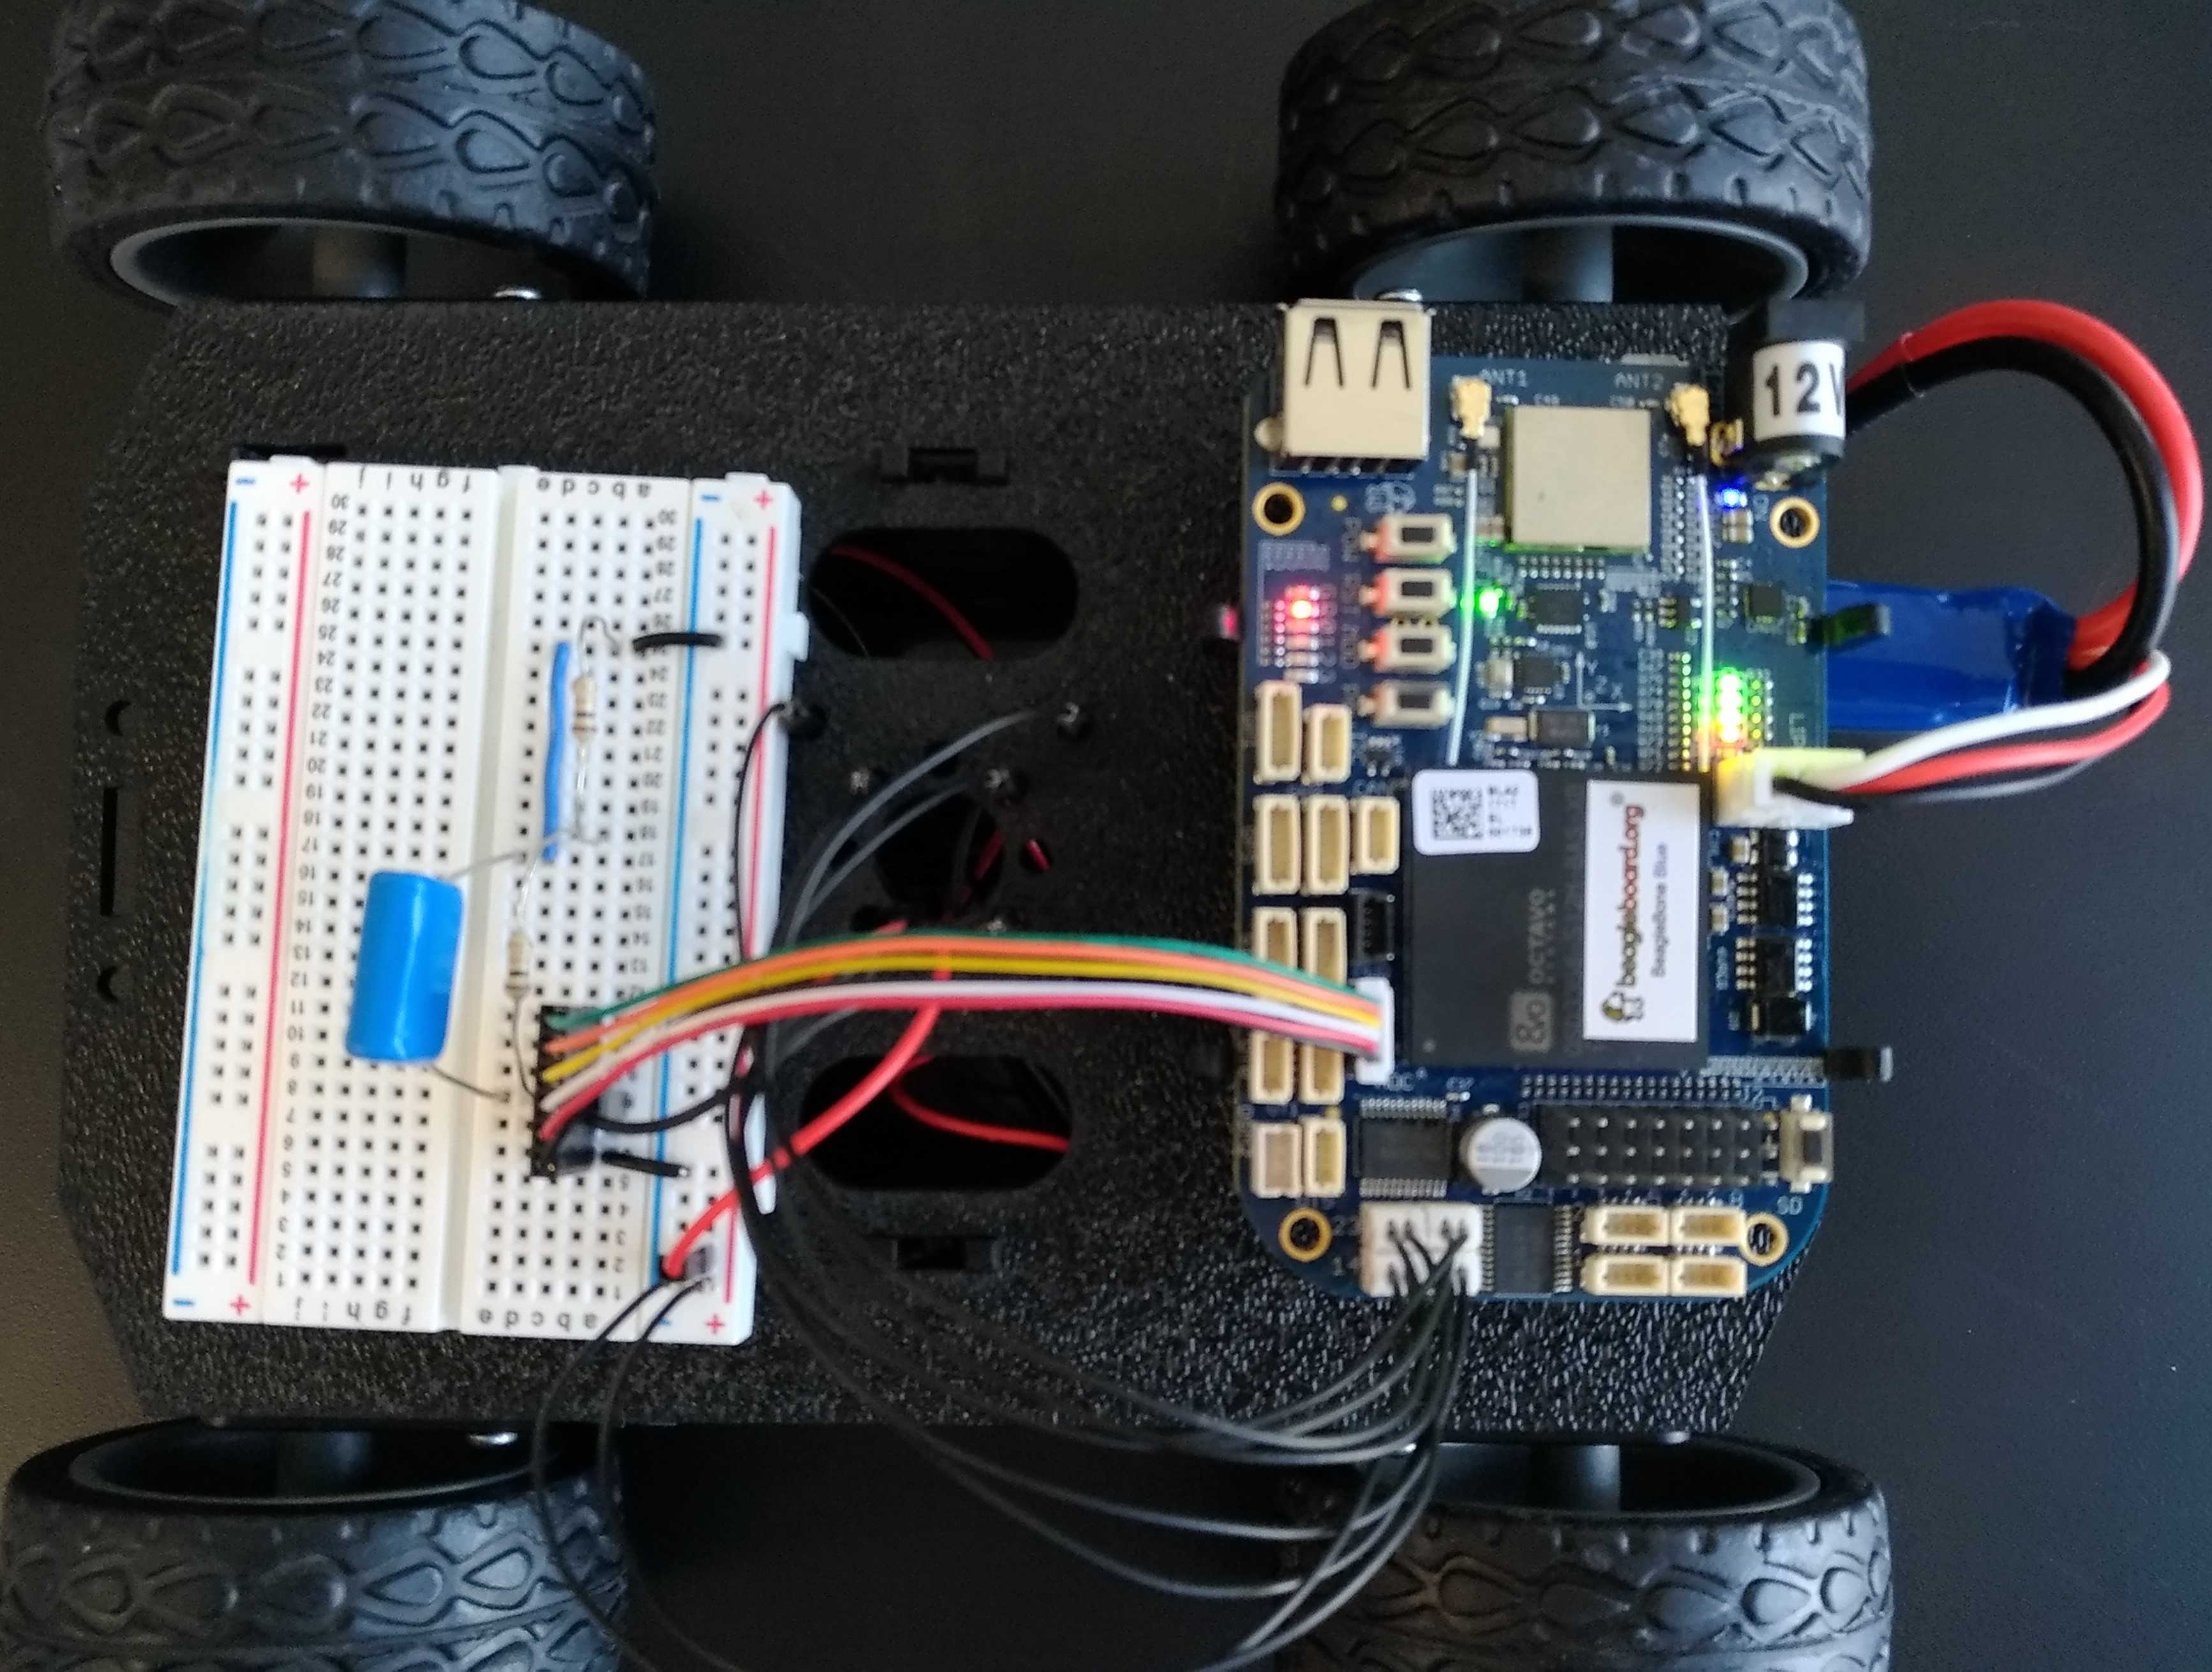
\includegraphics[scale=0.07]{figs/beaglebone/notConnectedSBC.jpg}
%     \caption{Embedded Computer Not Connected}
%     \label{fig:not_connected_bb}
% \end{figure}

% Figure~\ref{fig:not_connected_bb} shows the embedded computer mounted on the robot chassis with the circuit shown on page 9. It can also be seen that the embedded computer lights up the on-board red LED when disconnected. Figure~\ref{fig:connected_bb} shows that the embedded computer lights up the green LED when it is connected as an extra indication of its connection status.

% \begin{figure}[H]
%     \centering
%     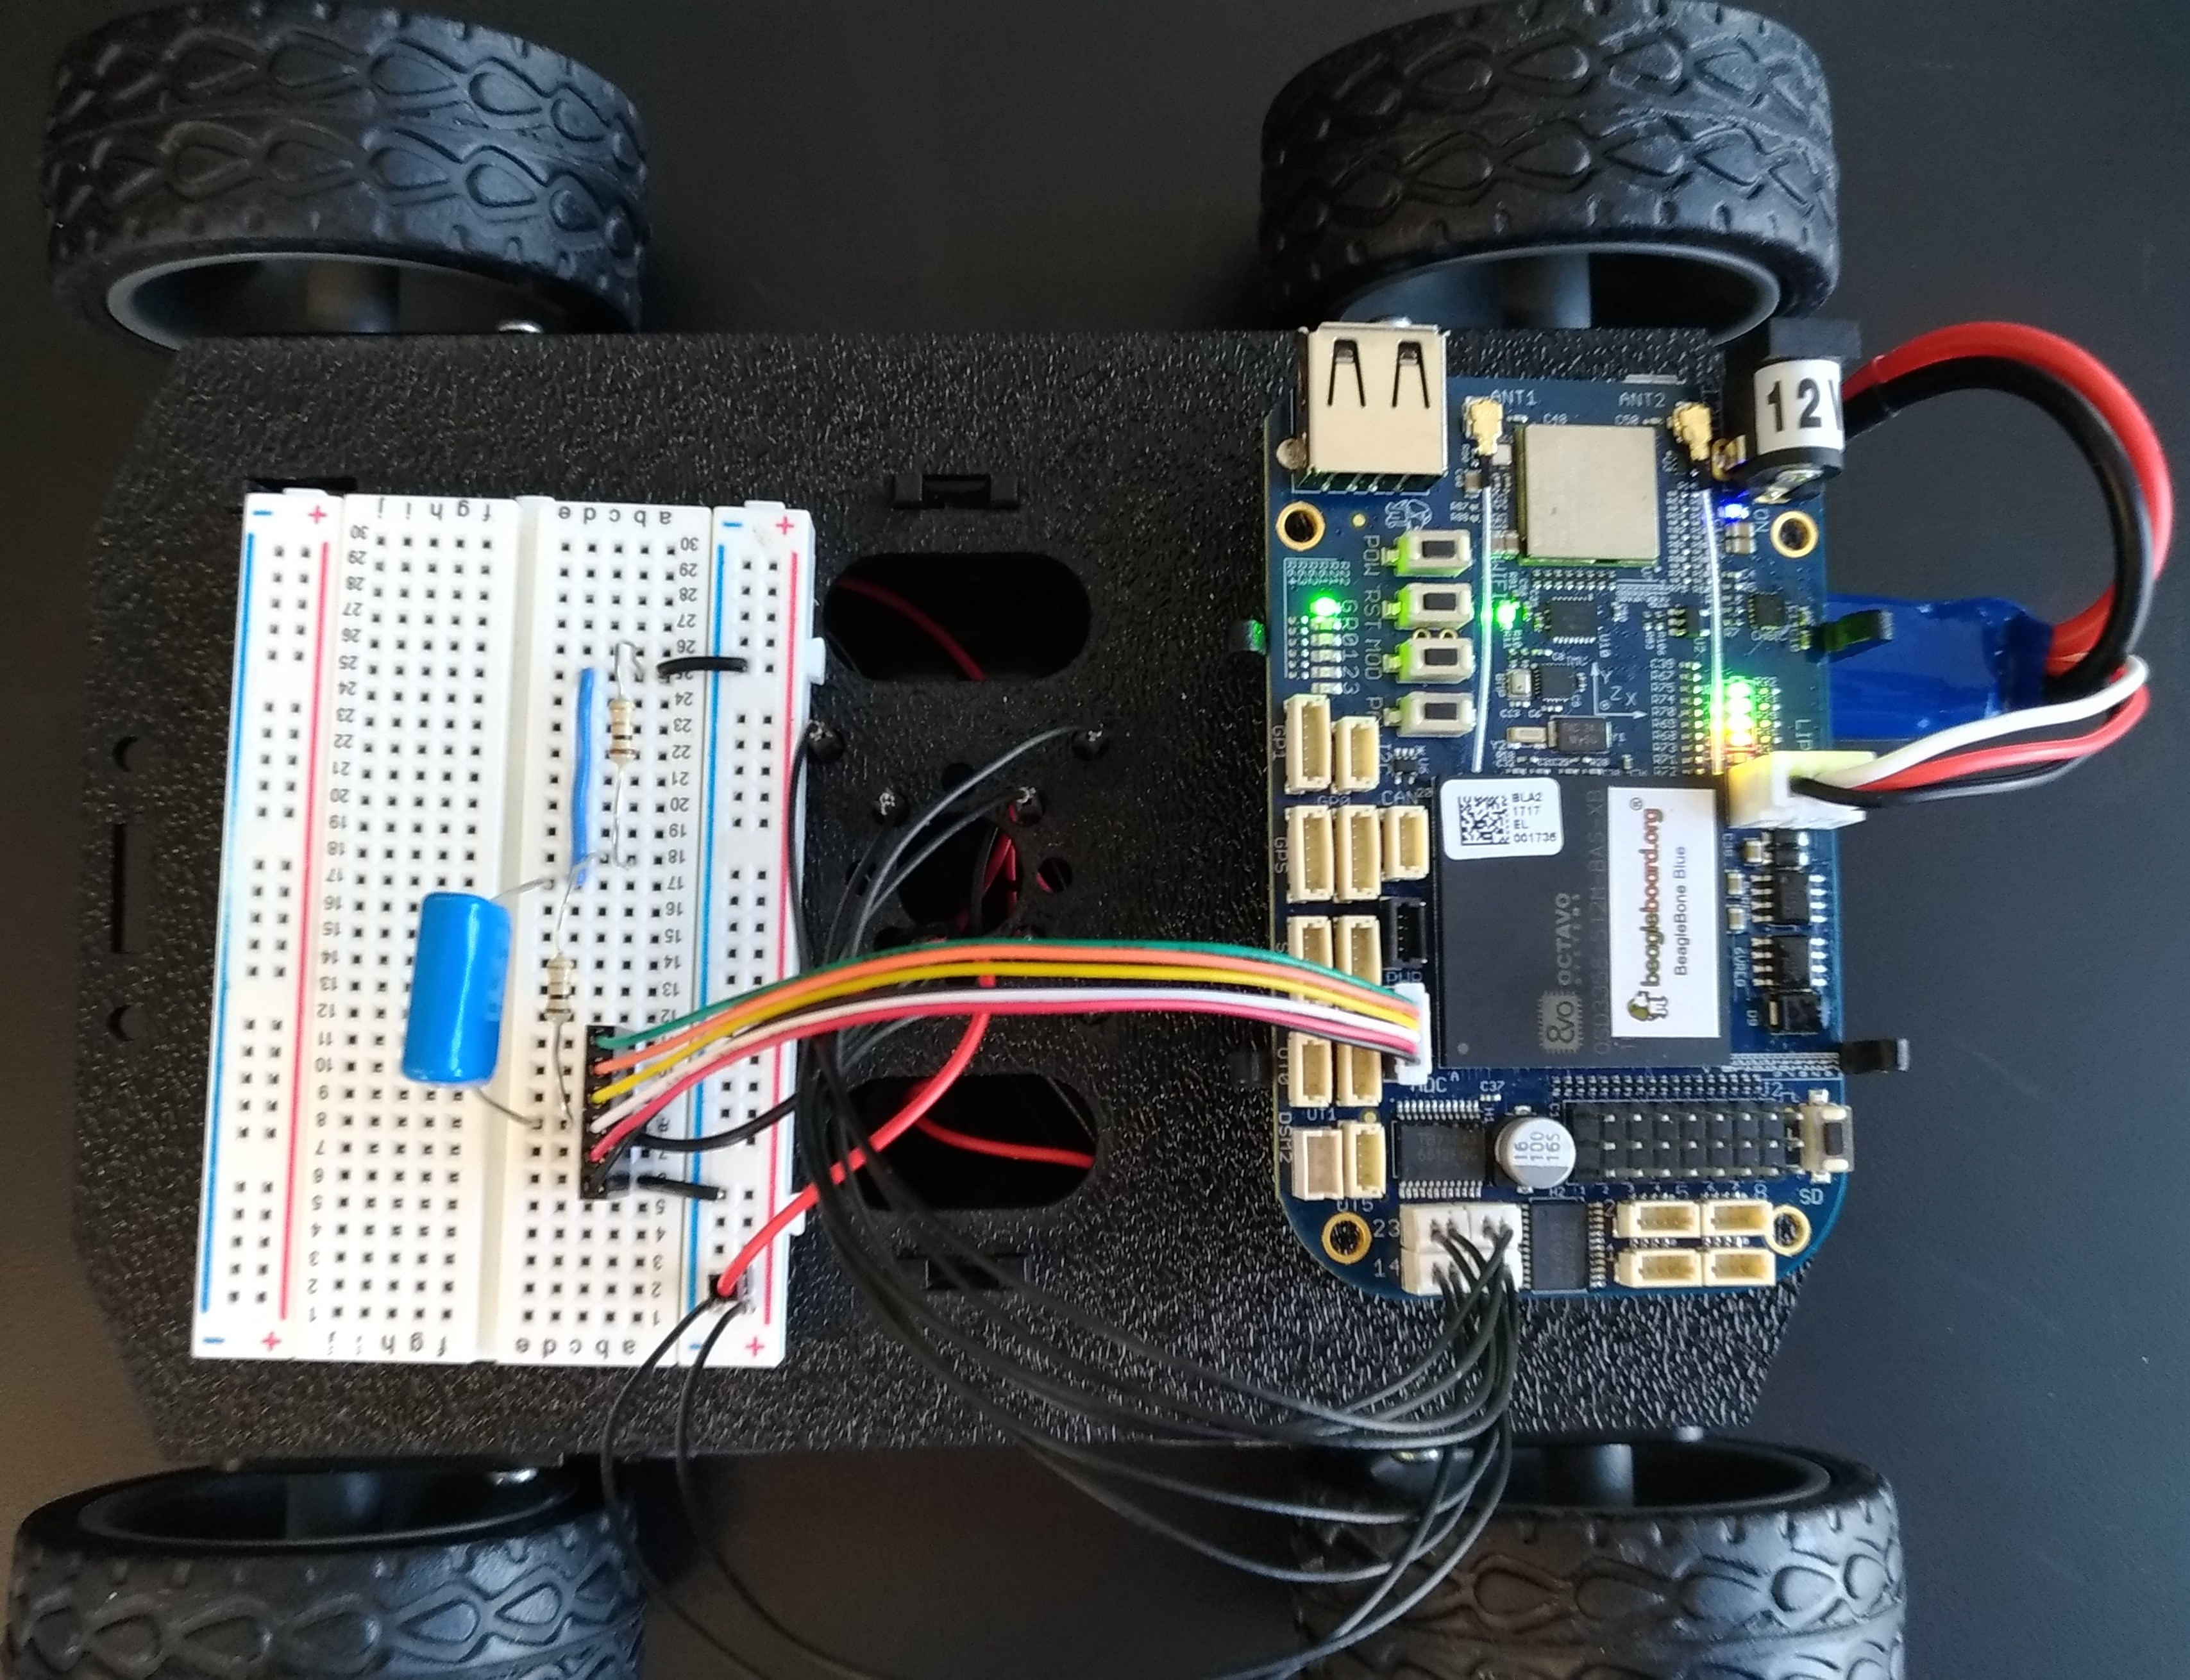
\includegraphics[scale=0.07]{figs/beaglebone/connectedSBC.jpg}
%     \caption{Embedded Computer Connected}
%     \label{fig:connected_bb}
% \end{figure}

% \begin{figure}[H]
%     \centering
%     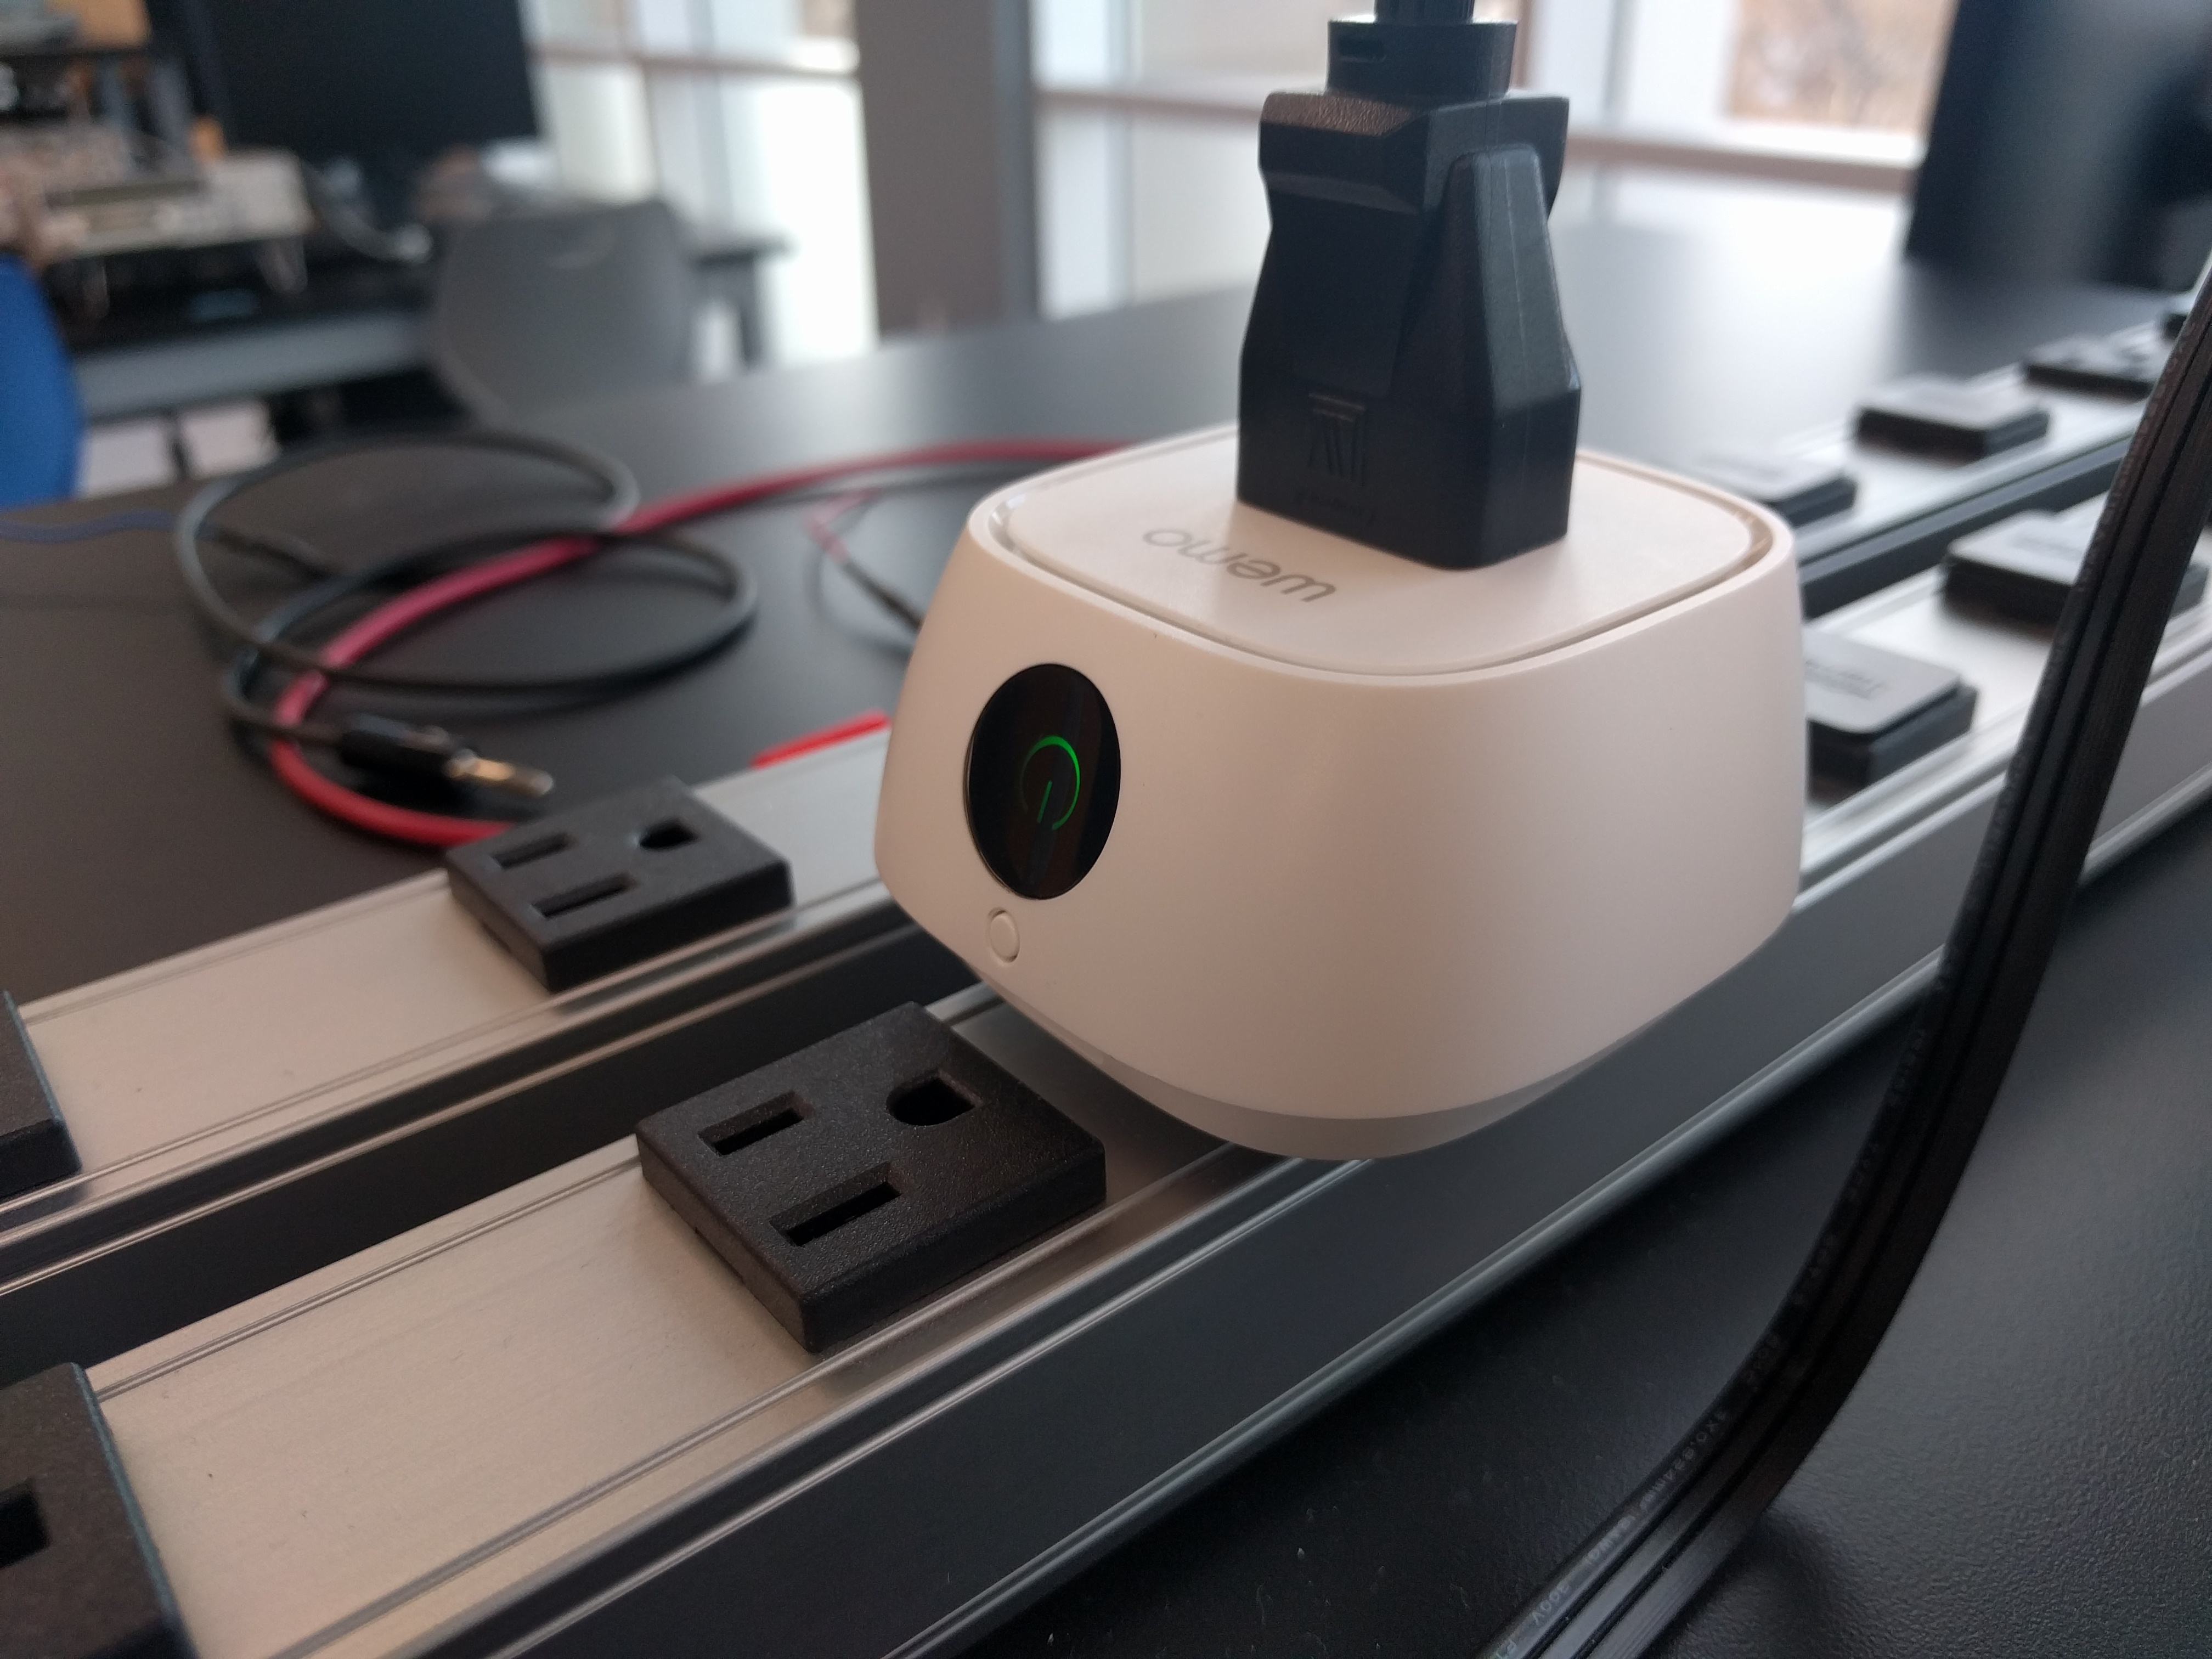
\includegraphics[scale=0.07]{figs/wemo/wemoView.jpg}
%     \caption{WeMo Insight Smart Plug}
%     \label{fig:wemo}
% \end{figure}

% The other supported device is the WeMo Insight Switch as seen in Figure~\ref{fig:wemo}. This device was easy to develop support for as it is meant for building energy management. It simply plugs into a 120 volt 3-prong outlet and any typical household appliance running on 120 volts can be plugged into it. Internal circuitry allows the WeMo to be controlled remotely (turn On/Off) and to record power usage of whatever it is plugged into.

% \begin{figure}[H]
%     \centering
%     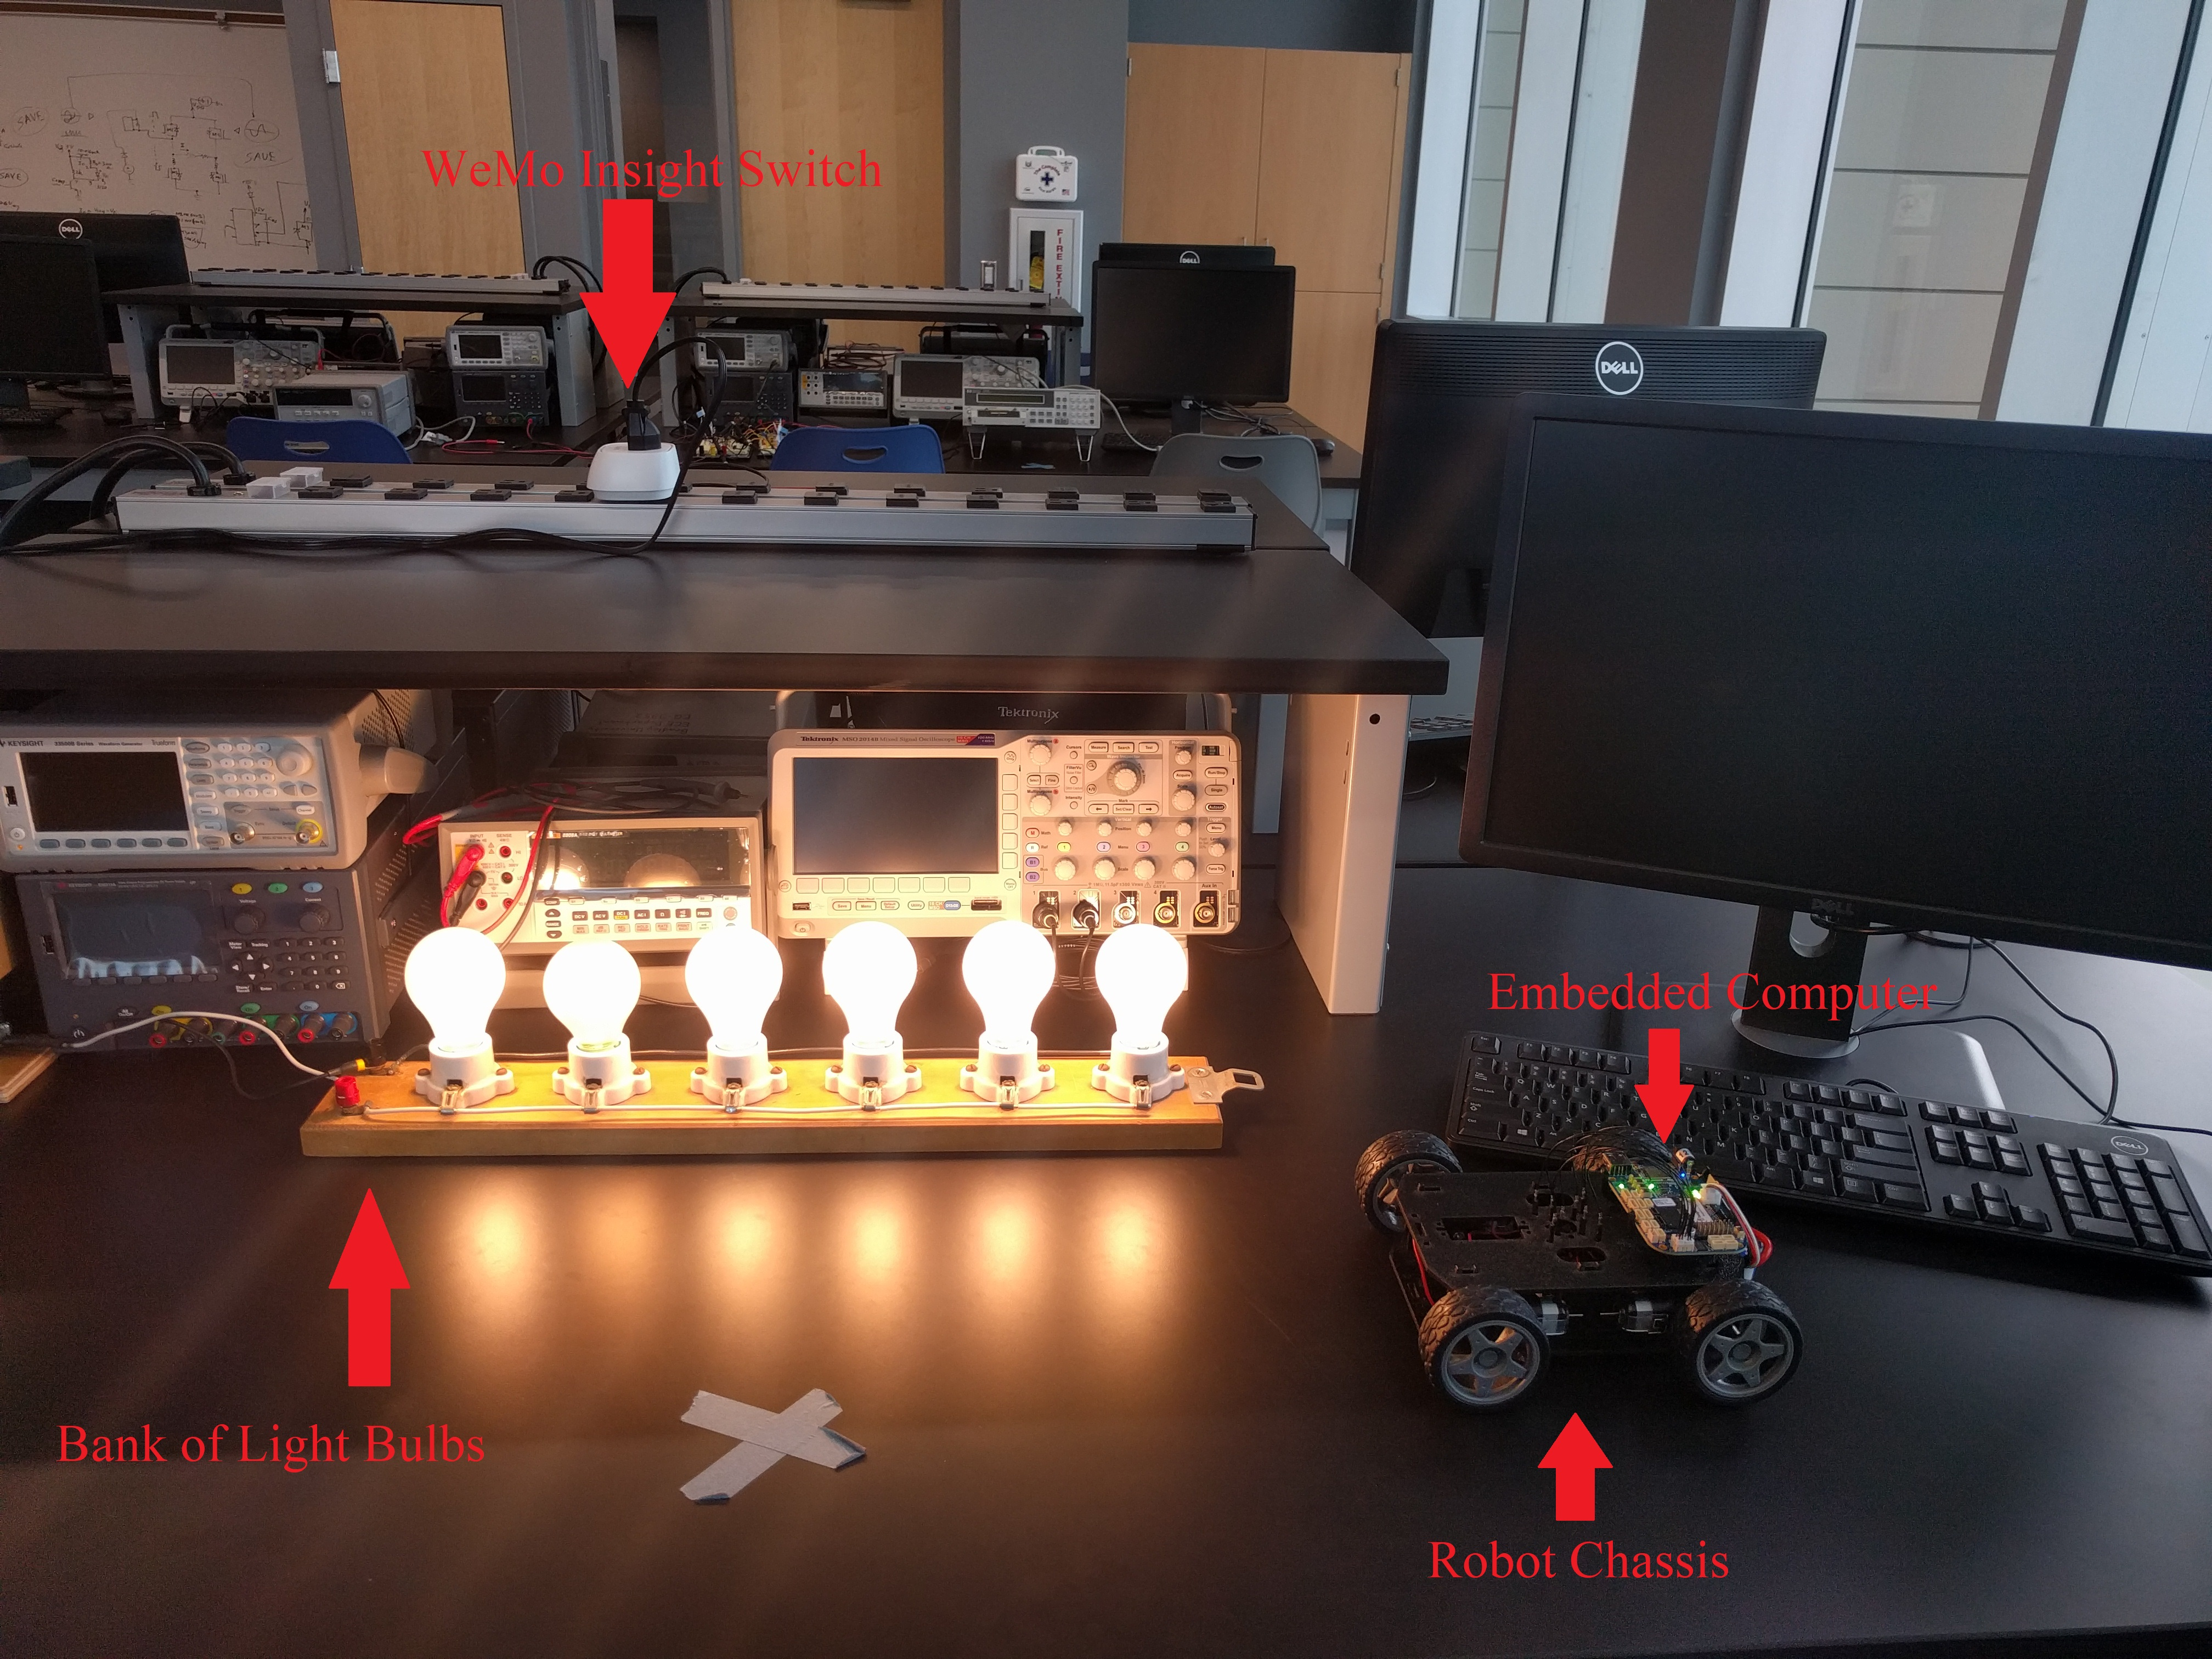
\includegraphics[scale=0.07]{figs/overallView.jpg}
%     \caption{Overall View}
%     \label{fig:overallView}
% \end{figure}

% In order to test these devices, we plugged a bank of 6 light bulbs into the WeMo
% Insight Switch as seen in Figure~\ref{fig:overallView}. The embedded computer's
% functionality was tested with the circuit and robot chassis described earlier.


\bibliographystyle{IEEEtran}
\bibliography{bib/references.bib}

\end{document}
